\documentclass[main]{subfiles} 
\graphicspath{{img/}}


\begin{document}

\section{Methodology}
A big difference between real estate and other publicly traded assets is that there is no centralized platform where offers can be tracked. 
In the case of asset classes such as bonds and equity this service is provided by multiple sources such as Bloomberg, Refinitiv and Morningstar.

Something similar is missing for the Swiss real estate market. 
Usually real estate on the various websites is presented as a list of single "tiles", 
along with a brief overview of the key data of the corresponding property (for reference see figure \ref{fig:listing}).
Normally there is no possibility to see the average cost per square meter in the ZIP code 
and no real way to compare similar estates.

Given that the data is neither available via an \acs*{api} nor through an already established database,
the decision was made to write an algorithm that scrapes the required data from a website.


\subsection{Choice of Website}

Whilst there exist numerous websites that act as middlemen between buyer and seller such as \verb|www.immoscout24.ch| and \verb|www.homegate.ch|,
all of them suffer from the same underlying problem mentioned in the introduction. 
Selecting and pricing real estate by clicking through listing after listing is cumbersome and inefficient.
Furthermore, with the data being split up over many websites, a buyer might not find his ideal new property, simply by looking on the wrong platform.

An attempt at creating a more transparent and efficient real estate market was made by Comparis. 
On their website, listings from many sources are aggregated and displayed according to their key characteristics.
However, also \verb|www.comparis.ch| does not offer tools for further analysis and does not readily display historical data,
except for increases or decreases in the price in percentage.

For the purpose of creating a database which provides a user with information on as many properties in a given area as possible, 
\verb|www.comparis.ch| is the ideal target for scraping data.


\subsection{Web Scraping}

When creating a web scraping application in Python, there are a number of packages and tools to choose from.
These modules include, but are not limited to \request, \beautifulsoup, \scrapy and last but not least, \selenium.
Each come with their advantages and disadvantages. 
The former two modules, \pkg[requests] and \beautifulsoup both come with the bonus of ease of use.
The latter two modules offer more functionality, but have a steeper learning curve.

After several attempts, the choice boiled down to a combination of \selenium and \scrapy.
This decision was based on the need to not only collect data on the "top level" of the listing (see \ref{fig:listing}), 
but also the information on the detail page of every single \acs*{url}.

\begin{figure}[htbp]
    \centerline{
        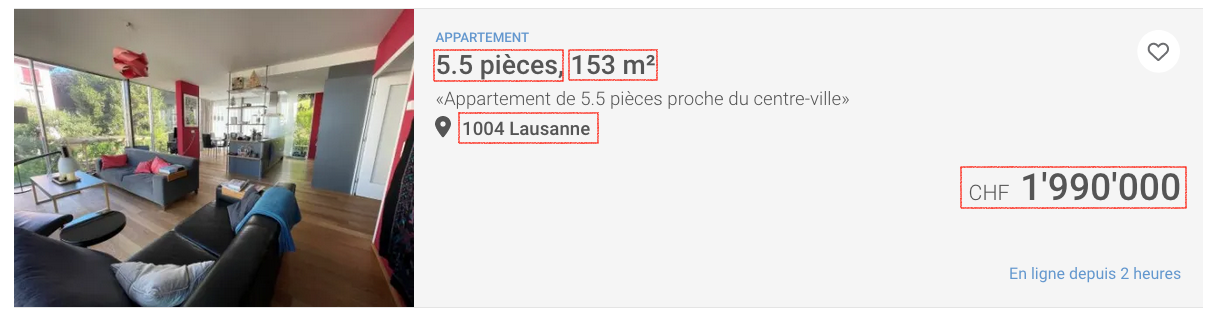
\includegraphics[width = 92mm]{prog_1.png}}
    \caption{Typical Listing on Comparis}
    \label{fig:listing}
\end{figure}

The need for more data was not the only factor that led to this choice.
Today's websites are populated with \js's that procedurally generate the content the user can see.
Generating further content may be triggered by simple actions such as scrolling on a page,
clicking a button, or by more complex actions such as hovering over a certain area or logging in somewhere.
For a web scraping service that relies on parsing \acs*{html} (such as \request and \beautifulsoup), this poses a major issue.
This is mainly because they cannot trigger a \js  by themselves and therefore cannot generate the source code that they could extract and parse.

\subsection{Scrapy}
Of the largest web scrapers available for python, \scrapy offers many options and usually serves the needs of larger scale web scraping projects.
The main feature that lead to the use of \scrapy for this project was the possibility of using a so-called spider.
The spider is set up by using the \pkg[scrapy genspider Comparis comparis.ch] command, 
along with several other files that allow granular customization of the spider.
In using a spider, a web scraper has to define a class (based on the class \pkg[scrapy.Spider], so it inherits all its attributes),
which tells \scrapy how and in which sequence to scrape which parts of a given website.

Information on websites is not readily available for scraping per se.
This entails that the output of the scraping process can be very disorganized and full of unwanted \acs*{html} tags.
Here \scrapy offers a very attractive solution, namely the \pkg[ItemLoader], which is defined as a class in the \pkg[items.py] file.
Whilst \pkg[ItemLoader] certainly adds to the steepness of the learning curve, it is a worthwhile endeavor, 
since the scraped data will come out clean already. 
\pkg[ItemLoader] "cleans" the data when it comes in, stores it while the spider is running, and generates an output based on the user's preference.

Furthermore, \scrapy can send many requests to a website at once, thus speeding up the data gathering process tremendously.
However, even when using all the request headers that a normal browser window sends to a website, 
the \scrapy spider's were constantly \acs*{ip}-blocked.

\begin{figure}[htbp]
    \centerline{
        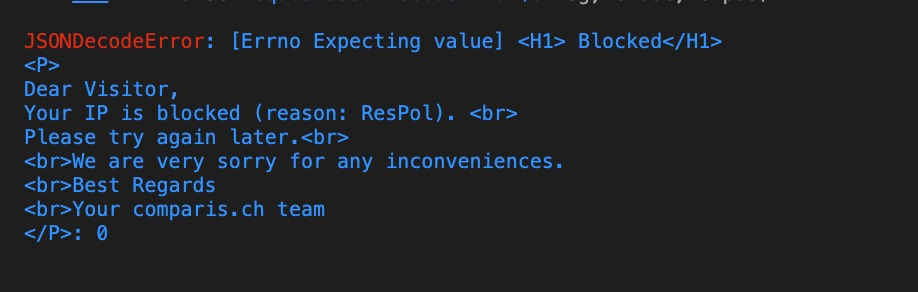
\includegraphics[width = 80mm]{prog_2.png}}
    \caption{IP block when running the spiders}
    \label{fig:block}
\end{figure}

\subsection{Selenium}
Whilst \scrapy works well with extracting data from the website's source code (expecially using \acsp*{xpath}), 
it is not possible to navigate \js heavy websites.
Furthermore, even with the implementation of rotating proxies, the \acs*{ip}-block could not be circumvented.
This is where \selenium comes in: \selenium allows a user to control any browser environment,
provided the corresponding driver has been installed.
Controlling a browser offers several advantages, the primary advantage being that the request comes from an actual browser,
which means it can hardly get blocked. 
The downside is that by sending the requests through a browser, the amount of requests per time is practically reduced to one.
This increased the runtime of the program drastically, however it ensured that the data collection was successful.

With some additional effort, combining \selenium with \scrapy can offer the best two worlds: reliable data gathering on the one hand,
and clean data extraction on the other hand.




\subsection{User platform}
To make the dataset scrapped from immoscout more user friendly we decided to build a graphical user interface(GUI).
This way the user will be able to search for a property within a certain price range, zip code or with specific features, 
instead or having to go through the full scrapped dataset.\par
We used the open source library tkinter to model the GUI. We chose this library as it is pre installed in python.
Moreover it is stable and flexible and provides simple syntax.\par
Tkinter is the perfect tool for this first prototype. However, if the project grows tkinter will not be powerful enough,
therefore we recommend switching to PyQT another UI or even REACT for a more professional look. 


\subsection{Structure}


\end{document}